\documentclass[../TDO1-O2.tex]{subfiles}%

\begin{document}
\section[s]"2"{Mirages}
% \enonce{%
% 	Cet exercice est une introduction à la propagation de la lumière dans un milieu
% 	non homogène. Le but est d'interpréter qualitativement les phénomènes de mirages
% 	(froid et chaud). Ces illusions d'optiques apparaissent lorsque l'indice de
% 	l'air varie assez rapidement avec l'altitude.
% }%
\begin{blocQR}
	\item \enonce{%
		Lorsque le sol est très «~chaud~», la température de l'air est
		d'autant plus élevée qu'il est proche du sol. Plus la température de
		l'air est élevée, moins son indice optique est élevé. On décompose
		l'atmosphère en N couches planes isothermes dont l'indice optique
		augmente avec l'altitude~:
		\[
			\forall k \in \Nb^* \quad\text{et}\quad 1 \leq k \leq N,
			\quad n_{k+1} > n_k
		\]
		\noindent
		\begin{minipage}{0.47\linewidth}
			\begin{center}
				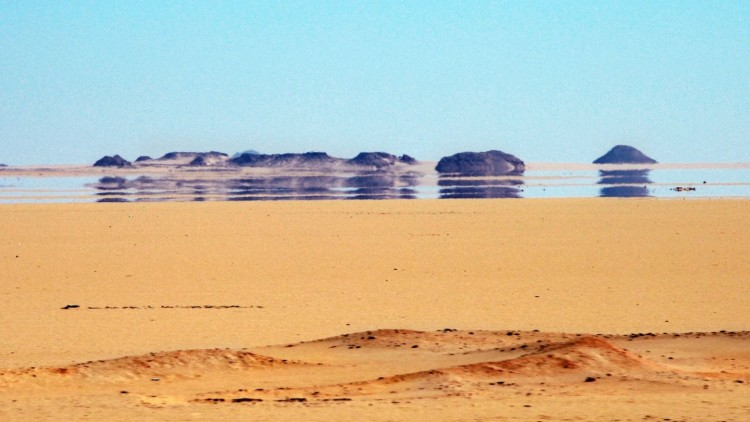
\includegraphics[width=\linewidth]{mirage_chaud}
				\captionof{figure}{Photo d'un mirage chaud}
				\label{fig:mir_chaud}
			\end{center}
		\end{minipage}
		\hfill
		\begin{minipage}{0.47\linewidth}
			\begin{center}
				\centering
				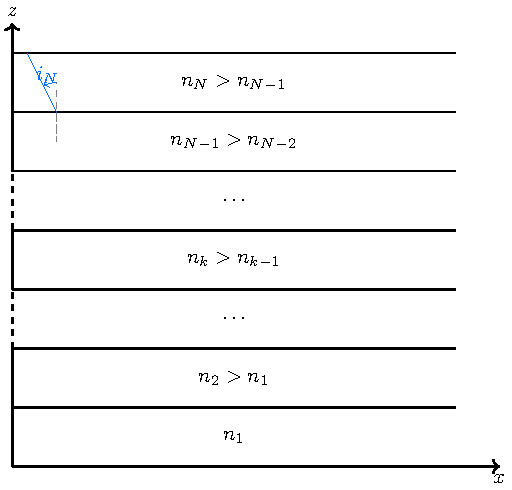
\includegraphics[height=5cm]{mirage_plain.pdf}
				\captionof{figure}{Modèle d'atmosphère stratifié}
				\label{fig:mirage_plain}
			\end{center}
		\end{minipage}
	}%
	\QR{%
		Montrer que $n_k\sin(i_k)$ est constant, où $k$ désigne la
		$k$-ième couche atmosphérique.
	}{%
		À chaque interface, $n_k\sin(i_k) = n_{k-1}\sin(i_{k-1})$~;
		notamment, avec $k=2$, on a $n_2\sin(i_2) = n_1\sin(i_1)$. Ainsi,
		tous les $n_k\sin(i_k)$ sont égaux.
	}%

	\QR{%
		Tracer les rayons réfractés par les couches d'air successives en
		faisant apparaître les angles d'incidence et de réfraction, puis
		montrer que pour un angle d'incidence initial suffisamment grand,
		une réflexion totale se produit.
	}{%
		Voir figure ci-après.\smallbreak
		À chaque «~dioptre~», on a $\sin(i_{\rm lim, k}) =
			\frac{n_{k-1}}{n_k}$. Sa valeur maximale est à $k=2$~:
		$\sin(i_{\rm lim,2}) = \frac{n_1}{n_2}$. Comme $n_k\sin(i_k)$
		est constant et que $n_k$ diminue, on sait que $i_k$
		augmente~: ainsi, si l'angle d'incidence $i_N$ est
		suffisamment grand, il y aura un $i_k$ supérieur à $i_{\rm
					lim,2}$ et donc réflexion totale.
	}%

	\QR{%
		Pour une variation continue de l'indice $n$, tracer qualitativement le
		trajet d'un rayon lumineux issu du ciel. Dans quel sens et direction sa
		trajectoire est-elle courbée~?
	}{%
		\begin{center}
			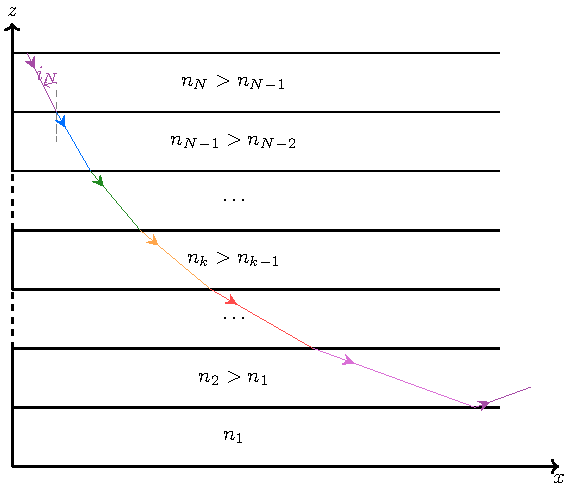
\includegraphics[width=.5\linewidth]{mirage}
			\captionsetup{justification=centering}
			\captionof{figure}{Rayons d'un mirage chaud. La trajectoire est courbée
				perpendiculairement vers le haut.}
			\label{fig:mirage}
		\end{center}
	}%

	\QR{%
		Interpréter alors le mirage chaud observé sur la photo ci-dessus.
		Faire un schéma.
	}{%
		Alors qu'on devrait voir le sable, les rayons venant du haut des
		collines sont déviés vers le haut~: on a l'impression de voir à
		travers la dune.
	}%

\end{blocQR}

\QR{%
	~
	\smallbreak
	\vspace{-15pt}
	\noindent
	\begin{isd}[righthand ratio=.35, interior hidden]
		Il arrive que la mer soit nettement plus «~froide~» que l'atmosphère. La
		température de l'air augmente alors avec l'altitude. Que peut-on observer si
		on regarde un bateau ou une île au loin~? Interpréter le
		mirage froid de la photo \ref{fig:mir_froid} ci-contre. Justifier par un
		schéma.
		\tcblower
		\begin{center}
			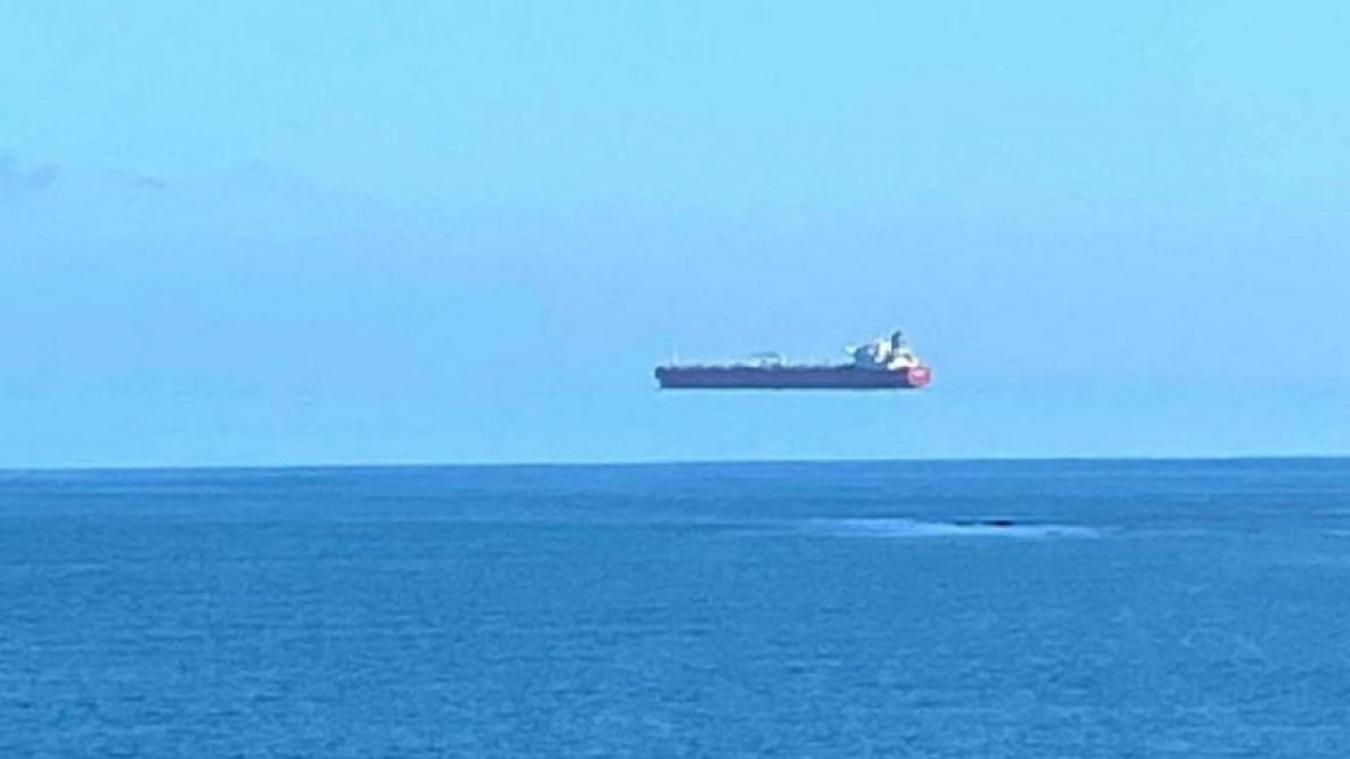
\includegraphics[width=\linewidth]{mirage_froid}
			\captionsetup{justification=centering}
			\captionof{figure}{Mirage froid.}
			\label{fig:mir_froid}
		\end{center}
		\vspace{-15pt}
	\end{isd}
	\vspace{-30pt}
}{%
	Cette fois ce sont les rayons dirigés vers le haut d'un objet lointain qui
	sont déviés vers le bas~: on a l'impression de voir des objets au-dessus du
	niveau de la mer. Schéma non fourni.
}%

\end{document}
